% ============================================================
%  RESEARCH PROPOSAL — A Comparative Study of GenAI-Generated and
%  Human-Authored Black-Box Test Suites
%  SE1907 -- Group 1, Software Testing (SWT301), FPT University
%
%  Structure follows the official course template:
%  "[Class]_[Group]_[Topic]_RESEARCH PROPOSAL.docx"
%  (Title fields -> Abstract -> 1..8 -> References)
%
%  Compile with XeLaTeX (required for Vietnamese diacritics in
%  author names). On Overleaf: Menu -> Compiler -> XeLaTeX.
%  Locally: xelatex Research_Proposal.tex  (run twice for the ToC/refs)
% ============================================================
\documentclass[12pt,a4paper]{article}

% ---------- Fonts / Vietnamese support ----------
\usepackage{fontspec}
\setmainfont{Times New Roman} % fallback: \setmainfont{Noto Serif} if unavailable

% ---------- Packages ----------
\usepackage[a4paper,margin=2.5cm]{geometry}
\usepackage{graphicx}
\usepackage{float}
\usepackage{caption}
\usepackage{booktabs}
\usepackage{longtable}
\usepackage{array}
\usepackage{tabularx}
\usepackage{enumitem}
\usepackage{xcolor}
\usepackage{hyperref}
\usepackage{fancyhdr}
\usepackage{amsmath}
\usepackage{amssymb} % for \checkmark in the appendix tables
\usepackage{titlesec}
\usepackage{tikz}
\usepackage{pdflscape} % landscape pages for the wide appendix tables

\hypersetup{
    colorlinks=true,
    linkcolor=black,
    citecolor=black,
    urlcolor=blue,
    pdftitle={A Comparative Study of GenAI-Generated and Human-Authored Black-Box Test Suites},
    pdfauthor={SE1907 Group 1}
}

\pagestyle{fancy}
\fancyhf{}
\fancyhead[L]{Research Proposal}
\fancyhead[R]{\leftmark}
\fancyfoot[C]{\thepage}
\renewcommand{\headrulewidth}{0.4pt}

\titleformat{\section}{\large\bfseries}{\thesection}{0.6em}{}
\titleformat{\subsection}{\normalsize\bfseries}{\thesubsection}{0.6em}{}

\newcolumntype{Y}{>{\raggedright\arraybackslash}X}

\begin{document}

% ============================================================
% TITLE BLOCK (matches the official template's field list)
% ============================================================
\begin{center}
    {\large \textbf{FPT UNIVERSITY}}\\[0.1cm]
    {\normalsize DEPARTMENT OF SOFTWARE ENGINEERING}\\[1cm]
    {\Large \textbf{RESEARCH PROPOSAL}}\\[0.8cm]
\end{center}

\begin{tabularx}{\textwidth}{lY}
    \textbf{Research title:} & A Comparative Study of GenAI-Generated and Human-Authored Black-Box Test Suites \\[0.3cm]
    \textbf{Sub-committee:}  & Software Testing \\[0.2cm]
    \textbf{Group name:}     & SE1907 -- Group 1 \\[0.2cm]
    \textbf{Authors:}        & Đặng Phước Vinh, Vũ Hà Ngọc Huyền, Phạm Nguyễn Quyền \\[0.2cm]
    \textbf{Mentor:}         & Nguyễn Nguyên Bình \\[0.2cm]
\end{tabularx}

\vspace{1cm}
\noindent\rule{\textwidth}{0.4pt}
\vspace{0.5cm}

% ============================================================
% ABSTRACT
% ============================================================
\section*{Abstract}
Black-box testing is a critical quality assurance practice, yet it remains labor-intensive, error-prone, and heavily dependent on tester expertise. This study conducts a rigorous empirical comparison of test suites generated by state-of-the-art Large Language Models (LLMs) against human-authored suites, organized as two methodologically distinct cohorts that are analyzed and reported \emph{separately} throughout. The \textbf{reproduced cohort} covers the three original applications of Kirinuki \& Tanno~\cite{b1} (Password Strength Checker, Unit Converter, Budget Planner): the published human (Human A--D) and ChatGPT (GPT-4) test suites are reused unchanged as a fixed baseline, and this study's own contribution is generating three \emph{additional} LLM suites (GPT-5.5, Claude 3.5 Sonnet, Gemini 3.1) against that same baseline. The \textbf{new cohort} covers two CLI applications authored specifically for this study (Library Fine Calculator, Task Manager): here both the AI suites (Sonnet 4.6, Gemini 3.1, ChatGPT-5.5) and the human suites (three third-year software engineering students, testing independently without AI assistance) are entirely original data collected by this team. Test viewpoints were manually extracted and mapped into a unified coverage matrix (\texttt{test perspective analysis 2.xlsx}), and coverage was measured using five quantitative metrics. Statistical significance was validated with an exact two-sided Wilcoxon signed-rank test computed via dynamic programming. Results show that modern LLMs significantly outperform human testers in viewpoint coverage (exact $p = 0.00002$ pooled across all categories), yet human testers still contribute unique boundary viewpoints that no AI model found. The Human+AI combined union achieves 98.1\%--100\% coverage across all five applications, confirming a strong synergistic potential for collaborative QA workflows. We conclude by proposing a two-phase QA process --- LLM-generated baseline followed by targeted human review --- as a practical adoption path for AI-assisted testing.

\vspace{0.3cm}
\noindent\textbf{Keywords:} Generative AI, Large Language Models, Software Testing, Black-Box Testing, Test Case Generation, Empirical Comparison, Test Viewpoint Coverage, Wilcoxon Signed-Rank Test.

\clearpage
\tableofcontents
\clearpage

% ============================================================
% 1. INTRODUCTION
% ============================================================
\section{Introduction}

\subsection{Background}
Black-box testing (specification-based testing) is a foundational software quality assurance (QA) practice in which test cases are designed purely from behavioral specifications, without knowledge of the internal implementation. This approach ensures that all externally observable behaviors --- including boundary values, invalid inputs, error handling, and state transitions --- are exercised by the test suite.

Traditionally, black-box test design has been entirely manual. Experienced testers analyze requirements documents, identify equivalence classes, boundary conditions, and error scenarios, then craft test cases accordingly. This process is time-consuming: in our study, the four professional developers used as the human baseline spent an average of \textbf{197.75 minutes} across the three replicated applications (60.25 min for Password Checker, 63.25 min for Unit Converter, 74.25 min for Budget Planner), yet still missed a significant fraction of viewpoints.

The emergence of Large Language Models (LLMs) trained on vast code repositories and natural language corpora has opened an unprecedented opportunity: these models can read a requirements specification and instantaneously generate comprehensive, structured test cases in natural language. The central question is no longer \textit{can} LLMs generate test cases, but \textit{how well} do they perform compared to humans across diverse applications and different levels of tester experience?

\subsubsection*{Problem statement}
Three core problems motivate this research:
\begin{enumerate}[leftmargin=1.2cm]
    \item \textbf{Stale benchmarks on older models.} The baseline study by Kirinuki \& Tanno~\cite{b1} benchmarked ChatGPT (GPT-4) only. Newer-generation models (GPT-5.5, Gemini 3.1, Claude 3.5 Sonnet) have not been rigorously benchmarked against identical human baselines under the same specifications and viewpoint-extraction methodology.
    \item \textbf{Undifferentiated human baselines.} Most comparative studies treat all human testers as a single ``human'' baseline. In reality, a professional developer with years of QA experience and a third-year student taking their first software testing course have fundamentally different cognitive testing strategies. Conflating these two groups obscures important insights.
    \item \textbf{Unmeasured synergy.} Even when studies show that LLMs achieve higher individual coverage than humans, they rarely quantify whether the two sources complement each other. If LLMs and humans cover \textit{different} blind spots, a combined Human+AI suite could achieve near-perfect coverage --- the most practically important finding for QA teams deciding how to adopt GenAI.
\end{enumerate}

\subsubsection*{Research Aim}
This study aims to empirically evaluate and statistically validate the black-box test coverage capabilities of modern GenAI LLMs versus human testers across five software specifications, and to measure the synergistic gain achieved by combining their test suites.

\subsubsection*{Research Objective}
\begin{itemize}[leftmargin=1.2cm]
    \item \textbf{O1a (reproduced cohort):} Generate three additional LLM test suites (GPT-5.5, Sonnet 4.6, Gemini 3.1) for the three original applications, and merge them into the same viewpoint matrix as the unmodified, published Human A--D and ChatGPT (GPT-4) suites from Kirinuki \& Tanno~\cite{b1} --- no new human data is collected for this cohort.
    \item \textbf{O1b (new cohort):} Author two original CLI specifications, generate test suites from three LLMs (Sonnet 4.6, Gemini 3.1, ChatGPT-5.5), and collect entirely new, independently-authored test suites from three third-year students (Student A--C) --- both the AI and human data for this cohort are primary data collected by this team.
    \item \textbf{O2:} Extract, categorize, and map all test viewpoints into a unified coverage matrix, keeping the reproduced and new cohorts in clearly separated sheets/sections at every stage.
    \item \textbf{O3:} Compute five quantitative metrics per tester per application: viewpoint coverage, category coverage, missing rate, unique contribution, and Human--AI union --- reported per cohort, never pooled across cohorts.
    \item \textbf{O4:} Validate the statistical significance of AI vs.\ human coverage differences via the exact Wilcoxon signed-rank test.
    \item \textbf{O5:} Analyze the student vs.\ professional performance gap and its implications for AI adoption in test automation workflows.
\end{itemize}

% ============================================================
% 2. LITERATURE REVIEW
% ============================================================
\section{Literature Review}

\subsection*{Overview of Existing Research}
Our review followed the PRISMA (Preferred Reporting Items for Systematic Reviews and Meta-Analyses) framework as introduced in the course methodology, searching arXiv, IEEE Xplore, and the ACM Digital Library with terms including \textit{LLM test generation}, \textit{black-box testing}, \textit{requirement-based test case}, and \textit{AI vs.\ human test suite}. Candidate papers were processed through the four PRISMA stages --- Identification, Screening, Eligibility, and Included --- before being retained as evidence for the final research design.

\begin{table}[H]
\centering
\caption{Selected related work}
\label{tab:literature}
\small
\begin{tabularx}{\textwidth}{p{2.6cm} c p{2.6cm} p{4.0cm} c}
\toprule
\textbf{Paper} & \textbf{Year} & \textbf{Method} & \textbf{Key Finding} & \textbf{Human Baseline} \\
\midrule
Kirinuki \& Tanno~\cite{b1} & 2024 & GPT-4, viewpoint coverage & ChatGPT covers basic viewpoints; professionals catch unique boundary cases & Yes (4 professionals) \\
Arora et al.~\cite{b2} & 2024 & RAG + LLM (industrial) & RAG improves domain accuracy of NL test scenarios & No (expert survey only) \\
Sami et al.~\cite{b3} & 2024 & React+Flask+OpenAI tool & Automates Gherkin writing; struggles with complex state logic & No \\
Tufano et al.~\cite{b4} & 2024 & TestGenEval benchmark & Best model (GPT-4o) averages only 35.2\% statement coverage on real repos & Yes (repo history) \\
Ferreira et al.~\cite{b5} & 2025 & AutoUAT + TestFlow (Cypress) & Helpful 95\% of the time; edge cases often missed & Yes (QA team) \\
\bottomrule
\end{tabularx}
\end{table}

\subsection*{Research Gaps}
\begin{itemize}[leftmargin=1.2cm]
    \item \textbf{Gap 1 (Model recency):} No study has benchmarked GPT-5.5, Gemini 3.1, and Claude 3.5 Sonnet together against a consistent human baseline under a reproducible viewpoint-extraction methodology.
    \item \textbf{Gap 2 (Baseline heterogeneity):} Existing studies do not separate the student tester cohort from the professional cohort, masking variance in human test quality that is critical for practical QA decision-making.
    \item \textbf{Gap 3 (Synergy quantification):} No study computes the union (Human+AI combined) coverage as a primary metric to measure how much the combined suite closes the gap toward 100\% coverage.
\end{itemize}

% ============================================================
% 3. RESEARCH SCOPE
% ============================================================
\section{Research Scope}

\subsection*{Research Questions}
\begin{itemize}[leftmargin=1.2cm]
    \item \textbf{RQ1:} How does the test viewpoint coverage (\%) of state-of-the-art LLMs compare to that of professional developers and software engineering students?
    \item \textbf{RQ2:} Is the difference in viewpoint coverage between AI and human test suites statistically significant, and at what granularity (application level vs.\ category level)?
    \item \textbf{RQ3:} To what extent do LLMs and human testers complement each other --- i.e., what is the Human+AI combined union coverage?
\end{itemize}

\subsection*{Scope of the Study}
\begin{table}[H]
\centering
\caption{Scope of the study}
\label{tab:scope}
\begin{tabularx}{\textwidth}{lY}
\toprule
\textbf{Dimension} & \textbf{Details} \\
\midrule
Applications (5) & Password Strength Checker, Unit Converter, Budget Planner (reproduced cohort); Library Fine Calculator CLI, Task Manager CLI (new cohort) \\
LLM models & Reproduced cohort: GPT-4 (reused) + GPT-5.5, Sonnet 4.6, Gemini 3.1 (newly generated). New cohort: Sonnet 4.6, Gemini 3.1, ChatGPT-5.5 (all newly generated) \\
Professional cohort (reused) & Human A--D --- published test suites from Kirinuki \& Tanno~\cite{b1}, reused unchanged; \emph{not} collected by this team \\
Student cohort (newly collected) & Student A--C (3rd-year SWE students) --- original test suites collected by this team for the 2 new CLI applications \\
Data source & \texttt{test perspective analysis 2.xlsx} --- single source of truth for all coverage data, with reproduced and new cohorts kept in separate sheets \\
Analysis scripts & \texttt{analyze\_viewpoints.py}, \texttt{wilcoxon\_test.py}, \texttt{author\_style.py}, \texttt{make\_charts.py} \\
\bottomrule
\end{tabularx}
\end{table}

% ============================================================
% 4. APPROACH AND METHOD
% ============================================================
\section{Approach and Method}

\subsection{Research Approach}
This is a quantitative empirical study. The methodology involves: (1) systematic test-suite generation and collection, (2) manual viewpoint extraction and categorization, (3) automated coverage computation via Python scripts, and (4) statistical significance testing.

\subsection{Data Preparation}

\subsubsection*{Dataset Sources}
Five natural language specifications were used as inputs. For the three reproduced applications, the original specifications from Kirinuki \& Tanno~\cite{b1} were used. For the two new CLI applications, original specifications were designed for this study (Section~\ref{sec:zenodo}).

\subsubsection*{Data Provenance: Reused vs.\ Newly Collected}
This is the single most important methodological distinction in the study design, and it is kept explicit through every later section, table, and figure:
\begin{itemize}[leftmargin=1.2cm]
    \item \textbf{Reproduced cohort (3 sheets --- Password Strength Checker, Unit Converter, Budget Planner):} the specifications, the four professional human test suites (Human A--D), and the ChatGPT (GPT-4) test suite are \emph{reused, unmodified,} from the published replication package of Kirinuki \& Tanno~\cite{b1}. This team's contribution for this cohort is limited to \emph{adding} three newly-generated LLM test suites (GPT-5.5, Sonnet 4.6, Gemini 3.1) against the same specifications, and re-scoring the resulting, extended matrix against the original, untouched human baseline. No new human test data was collected for these three applications.
    \item \textbf{New cohort (2 sheets --- Library Fine Calculator, Task Manager):} both the specifications and every test suite --- three LLMs \emph{and} three third-year students --- are original data produced for this study. This is a self-contained comparison of \emph{new models vs.\ new (student) human testers}, with no data inherited from prior work.
\end{itemize}
Because the two cohorts differ in provenance (secondary/reused data vs.\ primary/newly collected data) as well as in human-tester profile (industry professionals vs.\ 3rd-year students), they are never pooled into a single ``AI vs.\ human'' statistic. Every result table and figure in Section~6 reports the Reproduced and New cohorts as two separate rows/panels, and the Wilcoxon tests in Section~4.4 are likewise computed and interpreted per cohort before any cross-cohort discussion.

All test case files follow a consistent naming convention: \texttt{[ModelName]\_[AppName]\_test\_cases.txt}. For example, an excerpt from \texttt{GPT-5.5\_Budget\_planner\_test\_cases.txt}:
\begin{quote}
\small\ttfamily
\# Test case 1\\[2pt]
Add income minimum boundary: This test case verify adding an income with the minimum valid amount.\\
Test Steps:\\[2pt]
- \`{}planner add-income 1 "freelance"\`{}\\
- Verify that the output is \`{}Income added: \$1 from source "freelance".\`{}
\end{quote}

\subsubsection*{Prompt Design: Stateful vs.\ Stateless Applications}
Unlike a single generic prompt applied uniformly to every application, this study --- following the same design logic as Kirinuki \& Tanno~\cite{b1} --- uses \emph{two} zero-shot prompt templates, selected per application according to whether the CLI tool carries internal state across commands. This distinction matters because a \emph{stateless} application (e.g., a password checker) produces one self-contained input/output pair per invocation, whereas a \emph{stateful} application (e.g., a budget planner) requires a \emph{sequence} of commands whose final output depends on all prior commands (add an income, add an expense, then check the balance). Using a single-shot ``input $\rightarrow$ expected result'' format for a stateful application would be unable to express such sequences, so a distinct ``Test Steps'' format is required. The application-to-prompt mapping used in this study (recorded in \texttt{spec\_use\_prompt.txt}) is:

\begin{table}[H]
\centering
\caption{Prompt template assigned to each specification}
\label{tab:prompt-mapping}
\begin{tabularx}{\textwidth}{lcY}
\toprule
\textbf{Specification} & \textbf{App type} & \textbf{Reason} \\
\midrule
Password\_strength\_checker\_spec.txt & Stateless & Single password in, single strength verdict out; no data persists between runs. \\
Unit\_converter\_spec.txt & Stateless & Single (value, from-unit, to-unit) in, single converted value out. \\
Library\_fine\_calculator\_cli\_spec.txt & Stateless & Each invocation computes one fine from CLI flags; no stored loan records. \\
Budget\_planner\_spec.txt & Stateful & Incomes/expenses accumulate across commands; totals depend on the full command history. \\
Task\_manager\_cli\_spec.txt & Stateful & Tasks persist across add/update/complete/delete commands; correctness depends on state built up over multiple steps. \\
\bottomrule
\end{tabularx}
\end{table}

\paragraph{Stateless prompt template} (\texttt{prompt\_for\_stateless\_apps.txt}), used for Password Strength Checker, Unit Converter, and Library Fine Calculator:
\begin{quote}
\small\ttfamily
Create at least 50 test cases necessary and sufficient to ensure the correct behavior of a command line application "\{name\}" with the following specifications.\\
For invalid input, an appropriate and descriptive error message you create should be output.\\[4pt]
Your output should be as follows (surround by code block):\\[4pt]
\# Test case \{id\}\\[2pt]
\{Test case name\}: This test case verify \{description\}\\
Input: \`{}<name> \{input\}\`{}\\
Expected result: \`{}\{result\}\`{}\\[4pt]
\{specification\}
\end{quote}

\paragraph{Stateful prompt template} (\texttt{prompt\_for\_statefull\_apps.txt}), used for Budget Planner and Task Manager --- identical to the stateless template except that it explicitly resets state at the start of each test case and defers verification to the end of a command sequence:
\begin{quote}
\small\ttfamily
Create at least 50 test cases necessary and sufficient to ensure the correct behavior of a command line application "\{name\}" with the following specifications.\\
It is assumed that no data exists at the start of each test case.\\
Verify the output only once at the end of the test steps.\\
For invalid input, an appropriate and descriptive error message you create should be output.\\[4pt]
Your output should be as follows (surround by code block):\\[4pt]
\# Test case \{id\}\\[2pt]
\{Test case name\}: This test case verify \{description\}\\
Test Steps:\\[2pt]
- \`{}<name> \{command\} \{input\}\`{}\\
- \`{}<name> \{command\} \{input\}\`{}\\
- ...\\
- Verify that the output is \{expected result\}.\\[4pt]
\{specification\}
\end{quote}

The two extra sentences in the stateful template --- \textit{``It is assumed that no data exists at the start of each test case''} and \textit{``Verify the output only once at the end of the test steps''} --- exist precisely to force each generated test case to be a clean, independently-runnable sequence (avoiding hidden dependencies between test cases) while still allowing the multi-step state build-up that stateful CLI behavior requires. Keeping this distinction identical to the reference paper's own prompt design (rather than collapsing everything into one generic prompt) ensures that any coverage difference observed between applications reflects the LLMs' testing ability, not an artifact of an ill-fitting prompt format.

\subsubsection*{Inclusion Criteria (Newly Collected Human Test Suites --- New Cohort Only)}
The following criteria governed the collection of the three student test suites (Student A--C) for the two new applications. They do not apply to the reproduced cohort's Human A--D suites, which were collected under Kirinuki \& Tanno's own protocol~\cite{b1} and are reused as published.
\begin{itemize}[leftmargin=1.2cm]
    \item Human participants must test without access to source code (true black-box setting).
    \item Test cases must reference at least one expected output from the specification.
    \item Test suites must be submitted before the AI-generated results are shared.
\end{itemize}

\subsubsection*{Exclusion Criteria (All Newly Generated/Collected Suites)}
\begin{itemize}[leftmargin=1.2cm]
    \item Test cases that are purely structural (e.g., unit tests referencing internal functions).
    \item Duplicate test cases within the same test suite.
\end{itemize}

\subsubsection*{Data Extraction}
For each test suite, every viewpoint was manually extracted and mapped into the Excel matrix. Consistent with the course measurement convention, a viewpoint cell was marked \textbf{OK} if the corresponding test suite contained \emph{at least one} test case explicitly addressing that viewpoint; otherwise the cell was left blank. The mapping was cross-reviewed by two researchers to minimize subjectivity bias.

For the three reproduced applications (Password Strength Checker, Unit Converter, Budget Planner), the Excel sheet uses the following column layout:

\begin{table}[H]
\centering
\caption{Excel column layout --- reproduced applications (15 columns)}
\label{tab:cols-repro}
\small
\begin{tabularx}{\textwidth}{cY}
\toprule
\textbf{Col.} & \textbf{Meaning} \\
\midrule
A--B & Category, Test Viewpoint \\
C--I & Human TC\#, GPT-5.5, AI TC\#, Sonnet 4.6, AI TC\#, Gemini 3.1, \textit{(blank)} \\
J--N & ChatGPT 4.0, Human A, Human B, Human C, Human D \\
O & Effective viewpoint? \\
\bottomrule
\end{tabularx}
\end{table}

For the two new applications (Library Fine Calculator, Task Manager), only three AI models and three students were included:

\begin{table}[H]
\centering
\caption{Excel column layout --- new applications (12 columns)}
\label{tab:cols-new}
\small
\begin{tabularx}{\textwidth}{cY}
\toprule
\textbf{Col.} & \textbf{Meaning} \\
\midrule
A--B & Category, Test Viewpoint \\
C--H & TC\#, Sonnet 4.6, TC\#, Gemini 3.1, TC\#, ChatGPT-5.5 \\
I--K & Student A, Student B, Student C \\
L & Effective viewpoint? \\
\bottomrule
\end{tabularx}
\end{table}

\subsection{Proposed Framework / System Design}
The analysis pipeline consists of four Python scripts operating on the single Excel data source:
\begin{itemize}[leftmargin=1.2cm]
    \item \texttt{analyze\_viewpoints.py} $\rightarrow$ coverage \%, union, unique, and miss rate per source per application.
    \item \texttt{wilcoxon\_test.py} $\rightarrow$ exact Wilcoxon signed-rank $p$-value via dynamic programming.
    \item \texttt{author\_style.py} $\rightarrow$ effective-viewpoint table (Basic vs.\ Extracted), mirroring the reporting style of Kirinuki \& Tanno's Table 2.
    \item \texttt{make\_charts.py} $\rightarrow$ generates Figures~\ref{fig:coverage-repro}--\ref{fig:diff} (cohorts plotted separately; see Section~6).
\end{itemize}

\subsection{Evaluation Method}

\subsubsection*{Coverage, Miss, and Union: Definitions and Intuition}
Every viewpoint $v$ in the matrix is a yes/no cell for a given source $s$ (an LLM or a human tester): $covered(v,s)=1$ if that source's suite contains at least one test case addressing $v$, and $0$ otherwise (Section~4.2, \textit{Data Extraction}). From this binary matrix we define:
\begin{align}
    Cov &= \frac{N_{covered}}{N_{total}} \times 100\% \label{eq:cov}\\
    Cov_{cat} &= \frac{N_{covered\,in\,cat}}{N_{total\,in\,cat}} \times 100\% \label{eq:covcat}\\
    Miss &= \frac{N_{total} - N_{covered}}{N_{total}} \times 100\% = 100\% - Cov \label{eq:miss}\\
    Union &= \frac{\left| \{\, v \mid \exists s \in (Human \cup AI),\, covered(v,s) \,\} \right|}{N_{total}} \times 100\% \label{eq:union}
\end{align}
Eq.~\eqref{eq:cov} is the coverage of a \emph{single} source (e.g., GPT-5.5 alone) over the whole application; Eq.~\eqref{eq:covcat} is the same ratio restricted to one category (e.g., only the ``Boundary Value'' rows), and is what drives the per-category gap in Figure~\ref{fig:diff}. Eq.~\eqref{eq:miss} is simply the complement of coverage and quantifies the risk left unaddressed by a single source. Eq.~\eqref{eq:union}, the \emph{union} coverage, is the most important formula for RQ3: it does not average individual coverages, but instead asks, for each viewpoint, ``did \emph{any} source in this group cover it?'' --- which is why AI union and Human union in Table~\ref{tab:cohort-summary} are always $\geq$ the best individual source in that group. Unique contribution is defined analogously as the count of viewpoints covered by \emph{exactly one} source and by no other source in either group.

Figure~\ref{fig:venn} illustrates how these quantities partition the full viewpoint set $N_{total}$ for a single application: the AI union and Human union are the two circles, their intersection is the ``common core'' (covered by both), each circle's exclusive area is that group's unique contribution, and any area outside both circles is the \textbf{blind spot} --- viewpoints missed by every source, AI and human alike. The Human+AI combined coverage (Eq.~\eqref{eq:union} applied to $Human \cup AI$) is exactly the area of the two circles together; $100\%$ combined coverage means the blind-spot region is empty.

\begin{figure}[H]
\centering
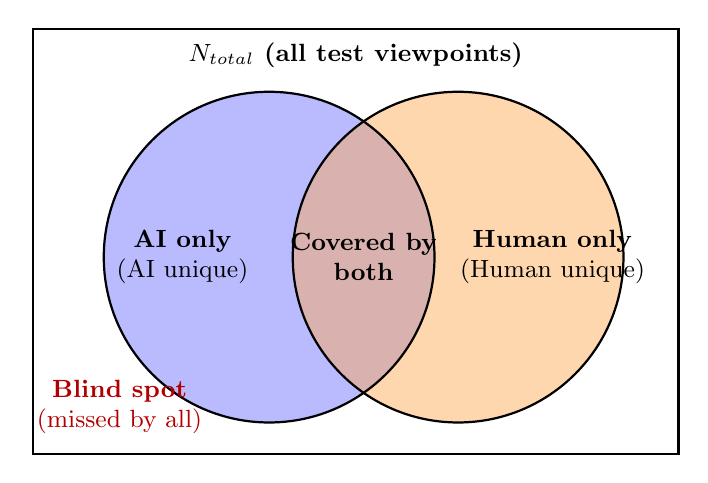
\begin{tikzpicture}[scale=1.0, every node/.style={font=\small}]
    \draw[thick] (0,0) rectangle (8.2,5.4);
    \node[anchor=north] at (4.1,5.35) {\textbf{$N_{total}$ (all test viewpoints)}};
    \begin{scope}[opacity=0.45]
        \fill[blue!60]   (3.0,2.5) circle (2.1);
        \fill[orange!70] (5.4,2.5) circle (2.1);
    \end{scope}
    \draw[thick] (3.0,2.5) circle (2.1);
    \draw[thick] (5.4,2.5) circle (2.1);
    \node[align=center] at (1.9,2.5) {\textbf{AI only}\\(AI unique)};
    \node[align=center] at (6.6,2.5) {\textbf{Human only}\\(Human unique)};
    \node[align=center] at (4.2,2.5) {\textbf{Covered by}\\\textbf{both}};
    \node[align=center,text=red!70!black] at (1.1,0.6) {\textbf{Blind spot}\\(missed by all)};
\end{tikzpicture}
\caption{How Cov, Union, unique contribution, and the blind spot partition $N_{total}$ for one application. Compare with the real per-cohort breakdowns in Figures~\ref{fig:synergy-repro} and~\ref{fig:synergy-new}.}
\label{fig:venn}
\end{figure}

\subsubsection*{The Wilcoxon Signed-Rank Test (Exact $p$-value via DP)}
The Wilcoxon test answers a different question than coverage alone: not ``how large is the AI--Human gap on average'', but ``is that gap \emph{consistently} in the same direction across independent pairs (applications or categories), more than chance would allow''. Let $d_i = Cov_{AI,i} - Cov_{Human,i}$ for each paired unit $i$ (an application or a category). After discarding ties ($d_i = 0$), rank $|d_i|$ from smallest to largest (tied absolute differences share the average of their ranks) and compute
\begin{equation}
    W^+ = \sum_{d_i > 0} \text{rank}(|d_i|), \quad W^- = \sum_{d_i < 0} \text{rank}(|d_i|), \quad W = \min(W^+, W^-).
\end{equation}
Intuitively, if AI and Human coverage were drawn from the same distribution, positive and negative differences should mix evenly, so $W^+$ and $W^-$ should be close to balanced ($\approx \text{Total}/2$ each); a very small $W$ means the ranks overwhelmingly favor one direction. The exact two-sided $p$-value is then computed by dynamic programming over all $2^{N_{usable}}$ possible $\pm$ sign assignments of the ranks --- i.e., every way the null hypothesis could have produced the observed ranks by chance. Ranks are doubled to integers to handle half-ranks from ties; let $r_j$ be the doubled rank of pair $j$, so the DP transition is
\begin{equation}
    dp[s] \mathrel{+}= dp[s - r_j], \quad \text{for } s = r_j, r_j+1, \ldots, \text{Total},
\end{equation}
where $dp[s]$ counts the number of sign assignments whose negative-rank sum equals $s$, and the exact $p$-value is the fraction of all $2^{N_{usable}}$ assignments at least as extreme as the observed $W$ on either tail:
\begin{equation}
    p = \frac{\displaystyle\sum_{s \le 2W} dp[s] + \sum_{s \ge \text{Total} - 2W} dp[s]}{2^{N_{usable}}}.
\end{equation}

\paragraph{Worked example (application level, $N=5$) --- reproduces Table~\ref{tab:wilcoxon}, row 1 exactly.} Using the five application-level averages already reported in Table~\ref{tab:cohort-summary}-style data (AI average and Human average per application, from \texttt{ket\_qua\_phan\_tich.txt}):

\begin{table}[H]
\centering
\caption{Step-by-step Wilcoxon ranking at the application level}
\label{tab:wilcoxon-worked}
\small
\begin{tabular}{lccccc}
\toprule
\textbf{Application} & \textbf{AI avg.} & \textbf{Human avg.} & \textbf{$d_i$ (pp)} & \textbf{$|d_i|$} & \textbf{Rank} \\
\midrule
Budget Planner            & 78.13\% & 64.38\% & $+13.75$ & 13.75 & 1 \\
Password Strength Checker & 75.73\% & 56.28\% & $+19.45$ & 19.45 & 2 \\
Unit Converter             & 83.65\% & 62.08\% & $+21.58$ & 21.58 & 3 \\
Library Fine Calculator    & 95.80\% & 66.67\% & $+29.13$ & 29.13 & 4 \\
Task Manager                & 86.23\% & 56.33\% & $+29.90$ & 29.90 & 5 \\
\bottomrule
\end{tabular}
\end{table}

All five differences are positive and no ties occur, so $W^+ = 1{+}2{+}3{+}4{+}5 = 15$ and $W^- = 0$, giving $W = \min(15,0) = 0$ --- exactly the $W^+=15.0,\,W^-=0.0$ reported for the application-level test in Table~\ref{tab:wilcoxon}. Doubling the ranks gives $r = \{2,4,6,8,10\}$ (Total $=30$). Because $W=0$, we need $\sum_{s\le 0} dp[s] + \sum_{s\ge 30} dp[s]$: the only subset of $\{2,4,6,8,10\}$ summing to $0$ is the empty set ($dp[0]=1$), and the only subset summing to $30$ is the full set ($dp[30]=1$), so the count is $1+1=2$, and
\begin{equation}
    p = \frac{2}{2^{5}} = \frac{2}{32} = 0.0625,
\end{equation}
which matches Table~\ref{tab:wilcoxon} exactly. This also demonstrates \emph{why} $p=0.0625$ is the smallest two-sided $p$-value obtainable with only 5 paired applications: it is reached whenever all differences point the same direction, regardless of their magnitude, because the DP only has $2^5=32$ possible sign patterns to distribute mass over. The category-level tests in Table~\ref{tab:wilcoxon} (Test 2, $N{=}20$; Test 3, $N{=}24$) follow the identical procedure over category-level $d_i$ instead of application-level $d_i$, computed automatically by \texttt{wilcoxon\_test.py}.

\subsection{Ethical Considerations}
The two cohorts raise different, cohort-specific ethical considerations. For the \textbf{new cohort}, all human data from student participants (Student A, B, C) is newly collected by this team and is fully anonymized; no personally identifiable information is stored in the analysis matrix, and participation was voluntary. For the \textbf{reproduced cohort}, the professional developer data (Human A--D) and the ChatGPT (GPT-4) suite are not collected by this team at all --- they are reused, with attribution, from the already-published baseline study~\cite{b1}, so no new consent or data-collection procedure was required on our part for that cohort. This research uses no sensitive datasets and poses no ethical risks.

% ============================================================
% 5. RESEARCH PLAN
% ============================================================
\section{Research Plan}
\begin{longtable}{p{0.6cm} p{4.3cm} p{4.3cm} p{2.2cm} p{1.8cm}}
\toprule
\textbf{No.} & \textbf{Task} & \textbf{Expected Output} & \textbf{Members} & \textbf{Target} \\
\midrule
\endhead
1 & Literature review \& PRISMA screening & Finalized literature matrix, 5 selected papers & All & Week 1 \\
2 & Specification preparation \& Zenodo collection & 5 spec files, 3 prompt template files & All & Week 2 \\
3 & Generate AI test cases (4 LLMs $\times$ 5 apps) & 20 AI test case files & All & Week 3 \\
4 & Collect human test suites (7 participants) & 7 human test case files & All & Week 3 \\
5 & Viewpoint extraction \& Excel matrix mapping & Completed \texttt{test perspective analysis 2.xlsx} & All & Week 4 \\
6 & Write \& validate Python analysis pipeline & \texttt{analyze\_viewpoints.py}, \texttt{wilcoxon\_test.py}, charts & All & Week 5 \\
7 & Statistical analysis \& interpretation & \texttt{wilcoxon\_ket\_qua.txt}, \texttt{ket\_qua\_phan\_tich.txt} & All & Week 5 \\
8 & Final report writing (Research Proposal) & Complete research proposal document & All & Week 6 \\
9 & Internal review \& revision & Revised proposal & All & Week 7 \\
\bottomrule
\caption{Research plan and task allocation}
\label{tab:plan}
\end{longtable}

% ============================================================
% 6. EXPECTED OUTCOMES
% ============================================================
\section{Expected Outcomes}

The following results were obtained by executing the Python analysis pipeline against \texttt{test perspective analysis 2.xlsx}. As established in Section~4.2 (\textit{Data Provenance}), the reproduced cohort (reused Human A--D / GPT-4 baseline) and the new cohort (newly-collected students) are two different comparisons and are therefore never drawn on the same chart --- each cohort gets its own pair of figures below, so that a bar chart never visually implies a single, homogeneous 5-application experiment.

\subsubsection*{Reproduced Cohort (Password, Unit Converter, Budget Planner)}

\begin{figure}[H]
\centering
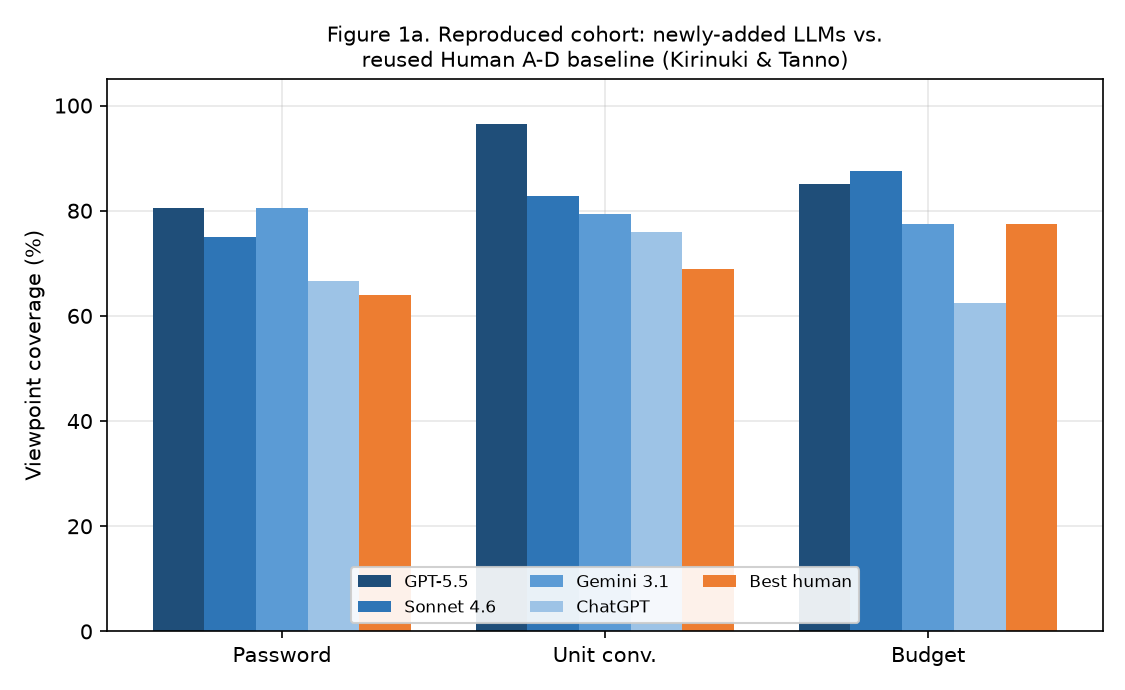
\includegraphics[width=0.72\textwidth]{../figures/fig1a_coverage_reproduced.png}
\caption{Reproduced cohort --- newly-added LLMs (GPT-5.5, Sonnet 4.6, Gemini 3.1) plus the original GPT-4, vs.\ the best of the reused Human A--D baseline, per application}
\label{fig:coverage-repro}
\end{figure}

Figure~\ref{fig:coverage-repro} shows that across the three reproduced applications, the newly-added AI models consistently and substantially outperform the best of the four reused professional testers. The coverage gap is largest in the Unit Converter (GPT-5.5: 96.6\%, best human: 69.0\%) and smallest in the Budget Planner (Sonnet 4.6: 87.5\%, Human D: 77.5\%) --- an area where systematic enumeration is a known LLM strength.

\begin{figure}[H]
\centering
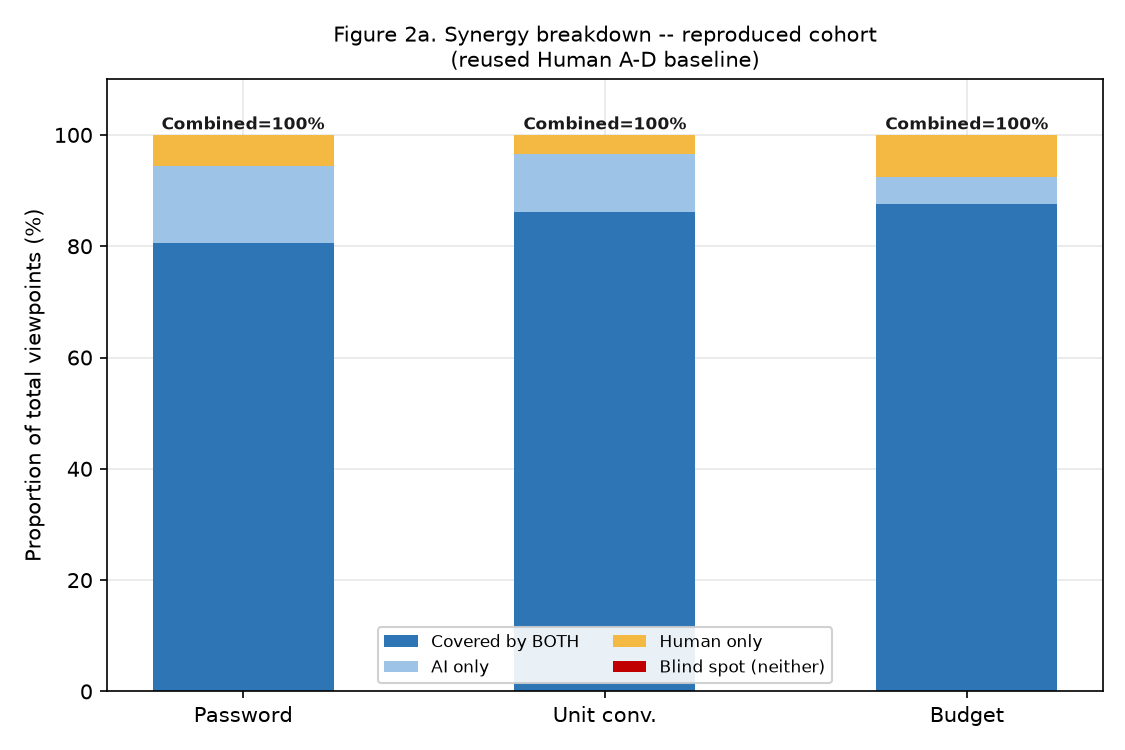
\includegraphics[width=0.72\textwidth]{../figures/fig2a_synergy_reproduced.png}
\caption{Synergy breakdown --- reproduced cohort (reused Human A--D baseline)}
\label{fig:synergy-repro}
\end{figure}

Figure~\ref{fig:synergy-repro} uses a stacked bar chart with four segments per application: \textbf{covered by both} (the common core), \textbf{AI only}, \textbf{human only}, and \textbf{blind spot} (missed by everyone). Key observations for this cohort:
\begin{enumerate}[leftmargin=1.2cm]
    \item \textbf{100\% combined union:} In the Password Strength Checker and Unit Converter, the combined (newly-generated AI) $\cup$ (reused human) union reaches a perfect 100\%; the AI-only and human-only segments are complementary.
    \item \textbf{Human supremacy in a specific domain:} Uniquely in the Budget Planner, the (reused) human union (95.0\%) exceeds the (newly-generated) AI union (92.5\%), reflecting the original professional testers' strength in mapping complex budget-calculation state transitions.
\end{enumerate}

\subsubsection*{New Cohort (Library Fine Calculator, Task Manager)}

\begin{figure}[H]
\centering
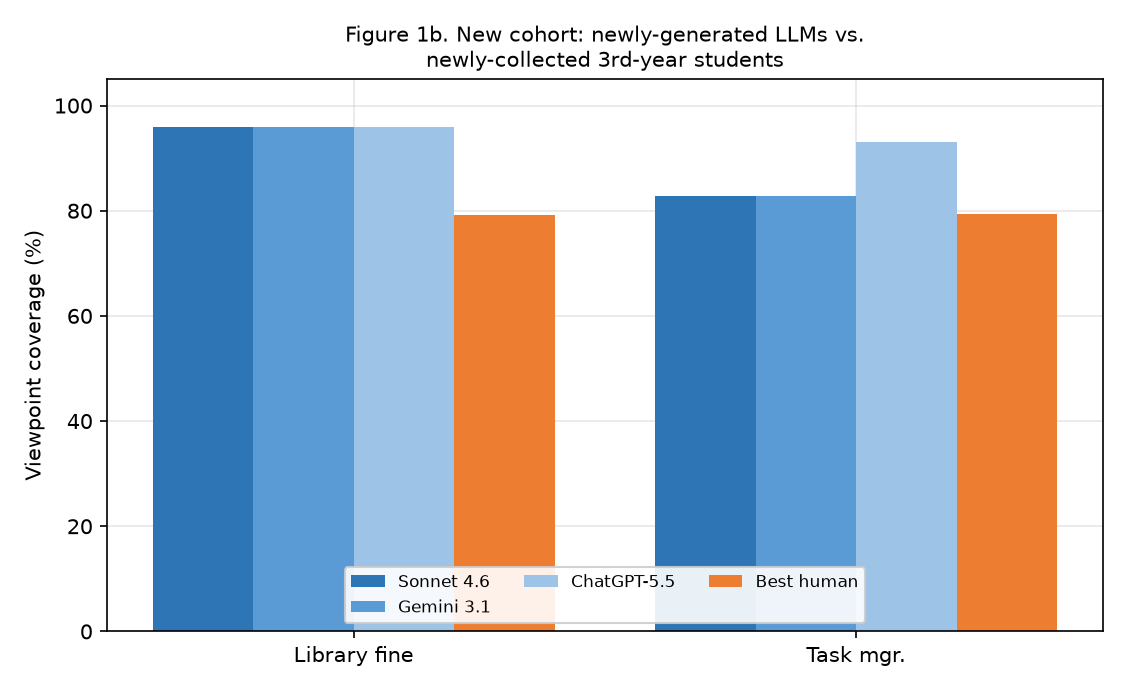
\includegraphics[width=0.72\textwidth]{../figures/fig1b_coverage_new.png}
\caption{New cohort --- newly-generated LLMs (Sonnet 4.6, Gemini 3.1, ChatGPT-5.5) vs.\ the best of the newly-collected 3rd-year students, per application}
\label{fig:coverage-new}
\end{figure}

Figure~\ref{fig:coverage-new} shows the same pattern holds in the entirely-original new cohort: newly-generated LLMs substantially outperform the best newly-collected student in both applications, and the gap is markedly larger here than in the reproduced cohort (Task Manager: ChatGPT-5.5 93.1\% vs.\ best student 79.3\%) because the student cohort includes one very low-performing outlier (Student C, discussed in Section~6's Expected Contributions).

\begin{figure}[H]
\centering
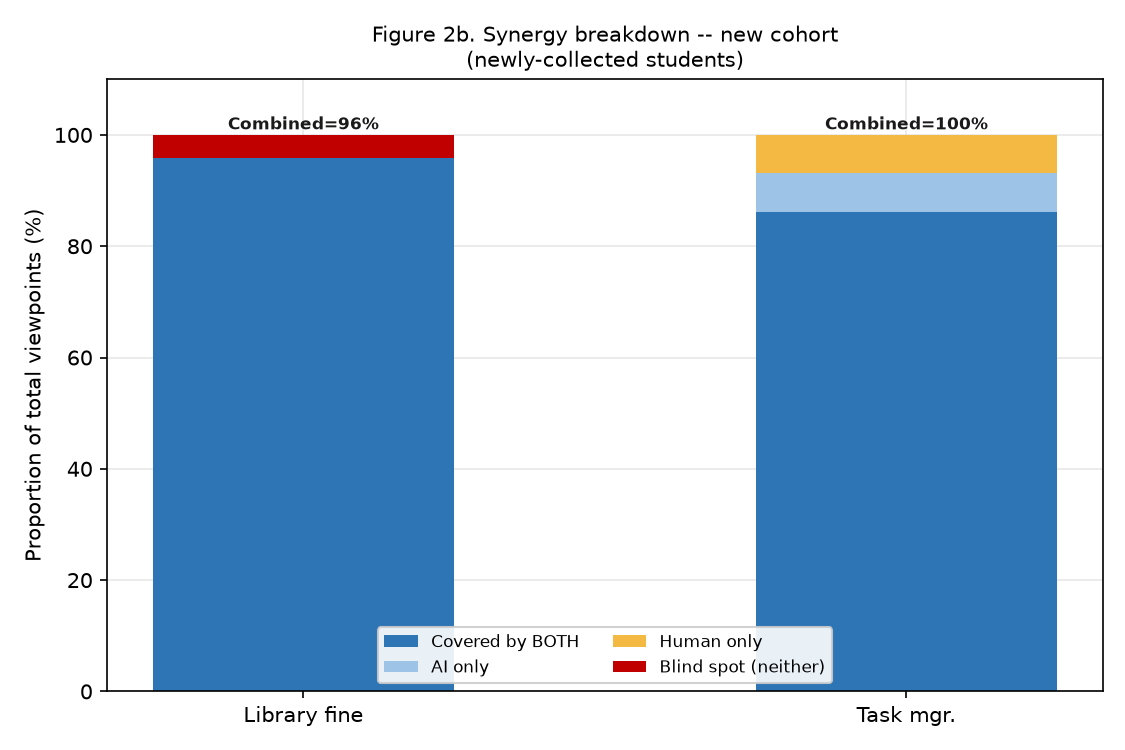
\includegraphics[width=0.72\textwidth]{../figures/fig2b_synergy_new.png}
\caption{Synergy breakdown --- new cohort (newly-collected students)}
\label{fig:synergy-new}
\end{figure}

Figure~\ref{fig:synergy-new} shows the same four-segment breakdown for the new cohort:
\begin{enumerate}[leftmargin=1.2cm]
    \item \textbf{100\% combined union (Task Manager):} the newly-generated AI-only and newly-collected human-only segments are complementary, closing the gap to full coverage.
    \item \textbf{Shared blind spot (Library Fine Calculator):} the combined union is only 96.0\%. Exactly \textbf{1 viewpoint} was missed by all 3 AI models \emph{and} all 3 student testers --- a genuine shared blind spot that Human+AI collaboration cannot recover, because neither source ever covered it.
\end{enumerate}

\subsubsection*{Pooled Category-Level View (Statistical Use Only)}

\begin{figure}[H]
\centering
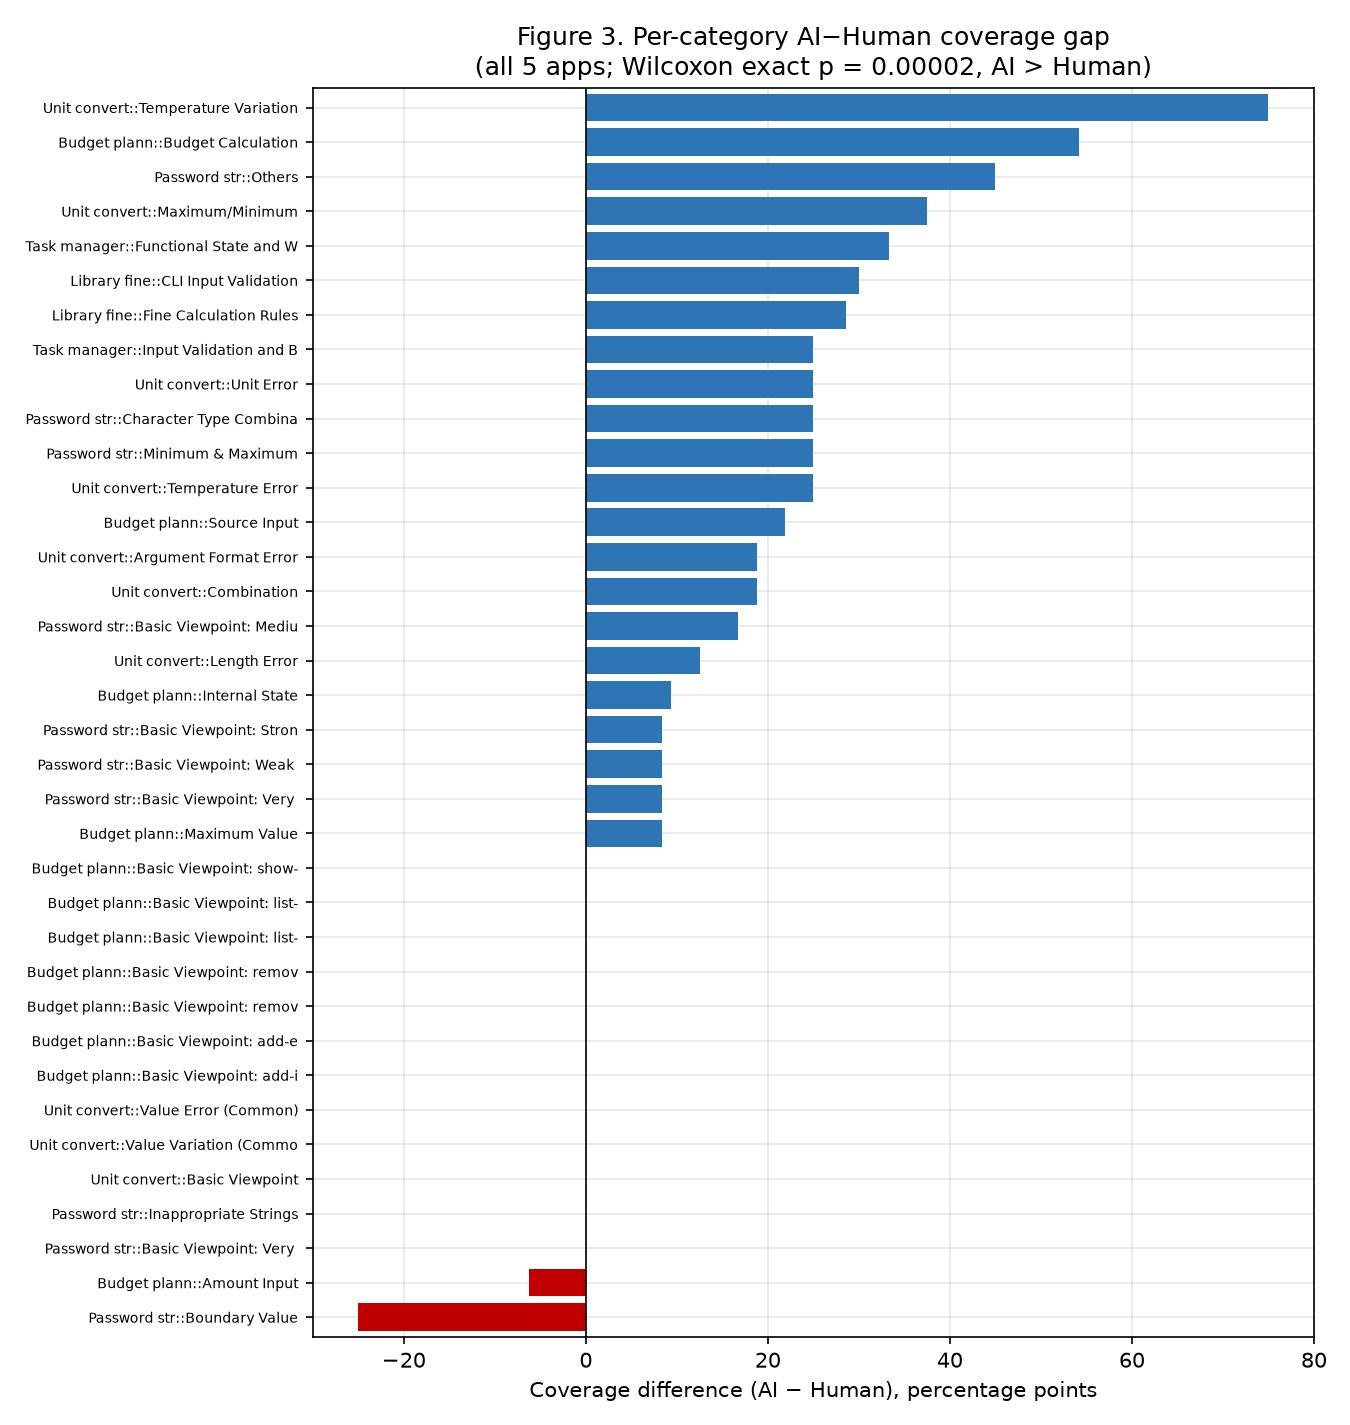
\includegraphics[width=0.85\textwidth]{../figures/fig3_category_diff.png}
\caption{Per-category AI--Human coverage gap, all 24 categories pooled from both cohorts}
\label{fig:diff}
\end{figure}

Unlike Figures~\ref{fig:coverage-repro}--\ref{fig:synergy-new}, Figure~\ref{fig:diff} \emph{intentionally} pools all 24 categories from both cohorts on one axis --- but only because this is exactly the pooled sample that feeds the ``Category (all 5 apps, $N{=}24$)'' row of the Wilcoxon test in Table~\ref{tab:wilcoxon} (Section~4.4), where pooling is a deliberate, explicitly-labeled statistical technique to gain test power, not a visual claim that the two cohorts are the same experiment. The two negative bars indicate the only categories (from either cohort) where humans outperformed AI: \textit{Password strength checker :: Boundary Value} ($-$25 pp, reproduced cohort) and \textit{Budget planner :: Amount Input} ($-$6.2 pp, reproduced cohort). In contrast, AI substantially outperformed humans in \textit{Unit converter :: Temperature Variation} ($+$75 pp, reproduced cohort) and \textit{Budget planner :: Budget Calculation} ($+$54.2 pp, reproduced cohort) --- areas of systematic enumeration and multi-condition state-transition reasoning.

\subsection*{Summary Table: Coverage by Cohort}
\begin{table}[H]
\centering
\caption{Coverage summary by cohort}
\label{tab:cohort-summary}
\resizebox{\textwidth}{!}{%
\begin{tabular}{lcccccc}
\toprule
\textbf{Cohort} & \textbf{Applications} & \textbf{AI Avg.} & \textbf{Human Avg.} & \textbf{AI Union} & \textbf{Human Union} & \textbf{Combined} \\
\midrule
Reproduced (professional) & Password, Unit, Budget & 81.1\% & 60.9\% & 94.3\% & 90.5\% & \textbf{100.0\%} \\
New (student) & Library Fine, Task Mgr & 89.2\% & 61.1\% & 94.3\% & 94.3\% & \textbf{98.1\%} \\
\bottomrule
\end{tabular}%
}
\end{table}

\subsection*{Statistical Significance Results}
\begin{table}[H]
\centering
\caption{Wilcoxon signed-rank test results}
\label{tab:wilcoxon}
\small
\begin{tabular}{lccccl}
\toprule
\textbf{Test} & \textbf{$N_{usable}$} & \textbf{$W^+$} & \textbf{$W^-$} & \textbf{Exact $p$} & \textbf{Conclusion} \\
\midrule
Application level ($N=5$) & 5 & 15.0 & 0.0 & 0.06250 & Not sig. (min.\ possible for $N{=}5$) \\
Category (reproduced, $N=20$) & 20 & 194.5 & 15.5 & 0.00027 & Significant \\
Category (all 5 apps, $N=24$) & 24 & 284.0 & 16.0 & 0.00002 & Highly significant \\
\bottomrule
\end{tabular}
\end{table}

With only five applications, the minimum achievable exact two-sided $p$-value is $2^{-4}=0.0625$; since all five AI means exceeded their human counterparts ($W^-=0$), we obtained exactly that mathematical floor. This is not a failed test, but a sample-size limitation. Pooling all 24 categories across the five applications yields an exact $p$-value of $0.00002$, with AI $>$ Human in 22 of 24 categories --- overwhelming evidence for the primary hypothesis.

\subsection*{Expected Contributions}
\begin{enumerate}[leftmargin=1.2cm]
    \item \textbf{A validated framework} for comparing LLM and human black-box test suites using reproducible, scripted viewpoint extraction and exact statistical testing.
    \item \textbf{A characterization of the professional vs.\ student gap:} student testers showed extreme variance (20.7\%--79.3\% coverage), suggesting GenAI is especially valuable as a quality floor for teams with inexperienced testers.
    \item \textbf{A synergistic QA workflow model:} since Human+AI combined coverage reaches $\geq$98.1\%, we propose a two-phase process --- (1) use LLMs to generate baseline coverage, then (2) use humans for targeted boundary and domain-specific review.
\end{enumerate}

% ============================================================
% 7. LIMITATIONS AND RISK
% ============================================================
\section{Limitations and Risk}

\subsection{Limitations}

\paragraph{Subjectivity in viewpoint extraction.} The mapping of raw test-case text to discrete viewpoints in \texttt{test perspective analysis 2.xlsx} was done manually. Despite cross-review by two researchers, subjective judgment was involved in deciding whether a test case implicitly ``covers'' a viewpoint --- a construct-validity threat. Future work should explore automated viewpoint extraction using NLP classifiers.

\paragraph{Scale of applications.} All five applications are small-scale, terminal-based CLI tools with well-defined specifications. The coverage advantages observed for LLMs may not generalize to large-scale, enterprise systems with implicit requirements or domain-specific jargon.

\paragraph{Viewpoint coverage $\neq$ fault detection.} This study measures only whether a tester \emph{addressed} a requirement aspect, not whether the corresponding assertion would actually catch a real bug. As emphasized in the course methodology, coverage answers ``did the suite mention this viewpoint?'' while a \emph{seeded-fault (mutation) analysis} answers ``can the suite catch a wrong implementation?''. A natural extension of this study would inject small, single-behavior mutants into the two new CLI specifications --- e.g., for the Task Manager, mutants such as \emph{default priority becomes ``low'' instead of ``medium''}, \emph{invalid priority ``urgent'' is accepted}, or \emph{task IDs start from 0 instead of 1} --- and compute a mutation score (killed mutants / total mutants) for each AI and human test suite. This was intentionally left out of the current scope due to the additional implementation and execution effort required, but is identified as the most direct next step to complement the viewpoint-coverage results reported here.

\paragraph{Student cohort size.} Only three students participated in the new-cohort experiment. This small sample size means the findings (especially the extreme variance, e.g., Student C at 20.7\%) may not generalize to the broader population of third-year software engineering students. A larger cohort ($N \geq 10$) would strengthen external validity.

\paragraph{LLM non-determinism.} LLM outputs are non-deterministic. The test suites generated in this study represent a single sampling of each model's output; repeated runs of the same prompt could yield different coverage scores.

\paragraph{Reused-baseline provenance (reproduced cohort only).} The Human A--D and ChatGPT (GPT-4) suites for the reproduced cohort are not freshly collected by this team; they are inherited unchanged from a study conducted in a different year, under a protocol this team did not control. Pairing that historical human/GPT-4 data with newly generated GPT-5.5/Sonnet~4.6/Gemini~3.1 suites is methodologically sound for viewpoint coverage (both sides are scored against the same fixed specification and rubric), but it does introduce a mild temporal-consistency threat that does not apply to the new cohort, where every suite --- AI and human alike --- was generated under identical, contemporaneous conditions. This is precisely why the two cohorts are never pooled into a single statistic in this report.

\subsection{Risk and Mitigation Strategies}
\begin{table}[H]
\centering
\caption{Risk analysis and mitigation strategies}
\label{tab:risk}
\small
\begin{tabularx}{\textwidth}{p{3.0cm} Y c Y}
\toprule
\textbf{Risk} & \textbf{Analysis} & \textbf{Impact} & \textbf{Mitigation} \\
\midrule
Publication bias & LLM research tends to over-report positive results; selected papers may inflate expected coverage benchmarks. & Medium & Measurements were cross-checked directly from the raw test-case files against the Excel matrix, independently of published claims. \\
Column-mapping errors in the Excel parser & Initial scripts mis-mapped \textit{Gemini 3.1} to a blank column instead of its actual column, corrupting statistics for Password and Unit Converter. & High & A full manual audit of all five sheet structures was performed and all column mappings were corrected; results were regenerated from scratch. \\
Heterogeneous human baseline \& data provenance & Mixing professional (reused, secondary) and student (newly collected, primary) data without distinguishing cohorts would produce a misleading average human benchmark and obscure that only 3 of the 5 applications' human data was collected by this team. & High & The two cohorts are strictly separated throughout all analyses, tables, and figures, and are reported independently at every stage; no pooled ``AI vs.\ human'' statistic spans both cohorts. \\
Overfitting the Wilcoxon test to category selection & Hand-picking the granularity of the test (application vs.\ category level) could introduce data-dredging concerns. & Medium & All three test levels are reported transparently, including the non-significant application-level test; no cherry-picking of results. \\
Prompt engineering bias & Different prompt templates could systematically advantage certain models. & Low & A single, standardized zero-shot prompt template was used for all four LLMs. \\
\bottomrule
\end{tabularx}
\end{table}

% ============================================================
% 8. SPECIFICATION COLLECTION FROM ZENODO
% ============================================================
\section{Specification Collection from Zenodo}
\label{sec:zenodo}

To prepare the input artifacts for the test-case generation phase, the study used the replication materials associated with Kirinuki \& Tanno~\cite{b1}. In their paper, the authors state that the application specifications, ChatGPT prompts, generated test cases, and extracted test viewpoints were shared via Zenodo at \url{https://zenodo.org/records/10476924}. This record was used as the primary source for two things, both limited to the reproduced cohort: (i) the software specifications of the three reproduced applications (Password Strength Checker, Unit Converter, Budget Planner), and (ii) the original human (Human A--D) and ChatGPT (GPT-4) test suites for those same three applications, which are reused unchanged as the fixed baseline described in Section~4.2. Only the specifications were needed as prompt input; the original human and ChatGPT-4 test cases were not regenerated or re-run.

The specification-collection process consisted of three steps. First, the team accessed the Zenodo record and identified the available specification files for the subject applications. Second, the collected specifications were reviewed and reformatted into a consistent requirement structure so they could be used as clear prompt inputs for the three \emph{newly added} LLMs (GPT-5.5, Sonnet 4.6, Gemini 3.1) --- the fourth model, ChatGPT (GPT-4), already had its test cases published in the same record and did not need to be re-prompted. Third, all AI-generated test cases (the three new ones, plus the reused GPT-4 set) were mapped back to the original specifications to evaluate requirement coverage, viewpoint coverage, boundary-value scenarios, and possible hallucinated or unsupported expected results.

For the two new CLI applications introduced in this study (Library Fine Calculator, Task Manager), no equivalent Zenodo materials existed; original specifications were authored by the team specifically to extend the replication study beyond the original three applications, following the same requirement structure used for the reproduced set.

This step is important because the quality of AI-generated black-box test cases depends strongly on the clarity and completeness of the input specification. By anchoring the reproduced cohort to the Zenodo materials connected to the reference paper, the study maintains traceability between the original research source, the extracted specifications, the LLM prompts, and the final test cases used for evaluation.

All specifications, prompts, test-case files, and analysis scripts used in this study are available at: \url{https://github.com/dpvinh30092005/research-testing-model-ai}.

% ============================================================
% REFERENCES
% ============================================================
\clearpage
\begin{thebibliography}{00}
\bibitem{b1} H. Kirinuki and H. Tanno, ``ChatGPT and Human Synergy in Black-Box Testing: A Comparative Analysis,'' \textit{arXiv preprint arXiv:2401.13924}, 2024.
\bibitem{b2} C. Arora, T. Herda, and V. Homm, ``Generating Test Scenarios from NL Requirements using Retrieval-Augmented LLMs: An Industrial Study,'' \textit{arXiv preprint arXiv:2404.12772}, Apr. 2024.
\bibitem{b3} A. M. Sami, Z. Rasheed, M. Waseem, Z. Zhang, H. Tomas, and P. Abrahamsson, ``A Tool for Test Case Scenarios Generation Using Large Language Models,'' \textit{arXiv preprint arXiv:2406.07021}, Jun. 2024.
\bibitem{b4} C. Tufano et al., ``TestGenEval: A Real World Unit Test Generation and Test Completion Benchmark,'' \textit{arXiv preprint arXiv:2410.00752}, Oct. 2024.
\bibitem{b5} M. Ferreira, L. Viegas, and J. P. Faria, ``Acceptance Test Generation with Large Language Models: An Industrial Case Study,'' in \textit{Proc.\ IEEE/ACM International Conference on Automation of Software Test (AST)}, 2025. arXiv:2504.07244.
\bibitem{b6} Course Lecture Slides, ``Collection \& Classification in Research,'' SWT301 --- Software Testing, FPT University, 2026.
\end{thebibliography}

% ============================================================
% APPENDIX — full per-viewpoint tables (landscape, wide tables)
% ============================================================
\clearpage
\appendix
\section{Extracted Test Viewpoints in Each Test Suite}
The detailed extracted test viewpoints covered by each test suite for all evaluated applications are presented below. All tables have been styled uniformly for optimal readability. Recall from Section~4.2 that Tables~\ref{tab:pwd_checker}--\ref{tab:budget_planner} (reproduced cohort) contain \emph{reused} Human A--D / GPT-4 columns alongside this study's newly-generated GPT-5.5 / Sonnet 4.6 / Gemini 3.1 columns, while Tables~\ref{tab:lib_fine}--\ref{tab:task_manager} (new cohort) contain only newly-generated data (three LLMs and three students).

\newgeometry{margin=1.5cm}
\begin{landscape}

% =========================================================
% TABLE I: PASSWORD STRENGTH CHECKER
% =========================================================
\begin{table*}[htbp]
\caption{Extracted Test Viewpoints from Password Strength Checker}
\label{tab:pwd_checker}
\centering
\renewcommand{\arraystretch}{1.1}
\footnotesize
\begin{tabular}{p{2.8cm} p{7.5cm} c c c c c c c c c}
\toprule
\textbf{Category} & \textbf{Test Viewpoint} & \textbf{GPT-5.5} & \textbf{Sonnet} & \textbf{Gemini} & \textbf{GPT-4} & \textbf{A} & \textbf{B} & \textbf{C} & \textbf{D} & \textbf{Eff?} \\
\midrule
Basic: Very Weak & 7 characters or fewer \& 1 type of character & \checkmark & \checkmark & \checkmark & \checkmark & \checkmark & \checkmark & \checkmark & \checkmark & \checkmark \\
& 7 characters or fewer \& 2 or more types of characters & \checkmark & \checkmark & \checkmark & & \checkmark & \checkmark & \checkmark & \checkmark & \checkmark \\
& 8 characters or more \& 1 type of character & \checkmark & \checkmark & \checkmark & \checkmark & \checkmark & \checkmark & \checkmark & \checkmark & \checkmark \\
\midrule
Basic: Weak & 8,9 characters \& 2 or 3 types of characters (exc. symbols) & \checkmark & \checkmark & \checkmark & \checkmark & \checkmark & \checkmark & \checkmark & \checkmark & \checkmark \\
& 8,9 characters \& 2 or more types of chars including symbols & \checkmark & \checkmark & \checkmark & \checkmark & & \checkmark & \checkmark & \checkmark & \checkmark \\
& 10 characters or more \& 2 or 3 types of chars (exc. symbols) & \checkmark & \checkmark & \checkmark & \checkmark & \checkmark & \checkmark & \checkmark & \checkmark & \checkmark \\
\midrule
Basic: Medium & 10,11 characters \& 2 types of characters including symbols & \checkmark & \checkmark & \checkmark & \checkmark & \checkmark & \checkmark & \checkmark & & \checkmark \\
& 10,11 characters \& 3 or more types of chars including symbols & \checkmark & \checkmark & \checkmark & \checkmark & & \checkmark & \checkmark & \checkmark & \checkmark \\
& 12 characters or more \& 2 types of characters including symbols & & \checkmark & \checkmark & \checkmark & \checkmark & & \checkmark & \checkmark & \checkmark \\
\midrule
Basic: Strong & 12$\sim$15 characters \& 3 types of characters including symbols & \checkmark & \checkmark & \checkmark & \checkmark & \checkmark & \checkmark & \checkmark & & \checkmark \\
& 12$\sim$15 characters \& 4 types of characters & \checkmark & \checkmark & \checkmark & & & \checkmark & \checkmark & \checkmark & \checkmark \\
& 16 characters or more \& 3 types of characters including symbols & \checkmark & & \checkmark & \checkmark & \checkmark & \checkmark & \checkmark & \checkmark & \checkmark \\
\midrule
Basic: Very Strong & 16 characters or more \& 4 types of characters & \checkmark & \checkmark & \checkmark & \checkmark & \checkmark & \checkmark & \checkmark & \checkmark & \checkmark \\
\midrule
Boundary Value & String length boundary values (exc. min and max lengths) & \checkmark & & \checkmark & & \checkmark & \checkmark & \checkmark & \checkmark & \checkmark \\
\midrule
Minimum \& Maximum & Minimum length (1) & \checkmark & \checkmark & \checkmark & & & & \checkmark & & \\
& Maximum length (100) & \checkmark & \checkmark & \checkmark & \checkmark & \checkmark & \checkmark & \checkmark & \checkmark & \checkmark \\
\midrule
Character Type Comb. & 4 ways to choose 1 type of character & \checkmark & \checkmark & \checkmark & \checkmark & & \checkmark & \checkmark & \checkmark & \checkmark \\
& 3 combinations of 2 types of characters excluding symbols & \checkmark & \checkmark & \checkmark & \checkmark & & \checkmark & \checkmark & \checkmark & \checkmark \\
& 3 combinations of 2 types of characters including symbols & \checkmark & \checkmark & \checkmark & \checkmark & & \checkmark & \checkmark & \checkmark & \checkmark \\
& 3 combinations of 3 types of characters including symbols & \checkmark & \checkmark & \checkmark & \checkmark & & \checkmark & \checkmark & \checkmark & \checkmark \\
\midrule
Inappropriate Strings & Failing by not providing a string & \checkmark & \checkmark & \checkmark & \checkmark & \checkmark & \checkmark & & \checkmark & \checkmark \\
& Failing by providing multiple strings & \checkmark & \checkmark & \checkmark & \checkmark & \checkmark & \checkmark & & \checkmark & \checkmark \\
& Failing by providing a string longer than the maximum length & \checkmark & \checkmark & \checkmark & \checkmark & \checkmark & \checkmark & \checkmark & \checkmark & \checkmark \\
& Failing by providing disallowed symbols & & & & \checkmark & & & & & \\
& Failing by providing multibyte/unicode characters & & & & \checkmark & \checkmark & \checkmark & \checkmark & \checkmark & \checkmark \\
& Including newline characters & & & & \checkmark & & \checkmark & & & \\
\midrule
Others & Linux command line "pipe" & \checkmark & \checkmark & & \checkmark & & & & & \\
& Repeating the same character & \checkmark & \checkmark & \checkmark & \checkmark & & & & & \\
& Randomly scattering types of characters evenly & \checkmark & & \checkmark & \checkmark & & & & & \\
& All kinds of lowercase letters & \checkmark & \checkmark & \checkmark & & & & \checkmark & & \\
& All kinds of uppercase letters & \checkmark & \checkmark & \checkmark & & & & \checkmark & & \\
& All digits & \checkmark & \checkmark & \checkmark & & & & \checkmark & & \\
& Using all symbols & \checkmark & \checkmark & \checkmark & \checkmark & & & \checkmark & \checkmark & \checkmark \\
& Testing the alphabet in reverse order & & & & \checkmark & & & & & \\
& Testing invisible unicode characters & & & & \checkmark & & & & & \\
& Failing by providing spaces at the beginning and end & & & & & & \checkmark & & & \\
\bottomrule
\end{tabular}
\end{table*}

% =========================================================
% TABLE II: UNIT CONVERTER
% =========================================================
\begin{table*}[htbp]
\caption{Extracted Test Viewpoints from Unit Converter}
\label{tab:unit_converter}
\centering
\renewcommand{\arraystretch}{1.1}
\footnotesize
\begin{tabular}{p{2.8cm} p{7.5cm} c c c c c c c c c}
\toprule
\textbf{Category} & \textbf{Test Viewpoint} & \textbf{GPT-5.5} & \textbf{Sonnet} & \textbf{Gemini} & \textbf{GPT-4} & \textbf{A} & \textbf{B} & \textbf{C} & \textbf{D} & \textbf{Eff?} \\
\midrule
Basic Viewpoint & For all units of length, appearing in either source or target... & \checkmark & \checkmark & \checkmark & \checkmark & \checkmark & \checkmark & \checkmark & \checkmark & \checkmark \\
& For all units of temperature, appearing in either source or target... & \checkmark & \checkmark & \checkmark & \checkmark & \checkmark & \checkmark & \checkmark & \checkmark & \checkmark \\
\midrule
Combination & Exhaustive coverage of two-unit combinations for length & \checkmark & \checkmark & \checkmark & \checkmark & \checkmark & \checkmark & \checkmark & \checkmark & \checkmark \\
& All units of length appear in both source and target & \checkmark & \checkmark & \checkmark & \checkmark & \checkmark & \checkmark & \checkmark & \checkmark & \checkmark \\
& Exhaustive coverage of two-unit combinations for temperature & \checkmark & \checkmark & \checkmark & \checkmark & \checkmark & \checkmark & & \checkmark & \checkmark \\
& All units of temperature appear in both source and target & \checkmark & \checkmark & \checkmark & \checkmark & \checkmark & \checkmark & \checkmark & \checkmark & \checkmark \\
\midrule
Unit Error & Conversion to a unit from a different category & \checkmark & \checkmark & \checkmark & \checkmark & \checkmark & \checkmark & \checkmark & \checkmark & \checkmark \\
& Conversion between the same units & \checkmark & \checkmark & \checkmark & \checkmark & & \checkmark & \checkmark & & \checkmark \\
& Providing a length unit that is not supported & \checkmark & \checkmark & \checkmark & \checkmark & & \checkmark & \checkmark & & \checkmark \\
\midrule
Value Variation & When the pre-conversion value is an integer & \checkmark & \checkmark & \checkmark & \checkmark & \checkmark & \checkmark & \checkmark & \checkmark & \checkmark \\
& When the pre-conversion value is a decimal & \checkmark & \checkmark & \checkmark & \checkmark & \checkmark & \checkmark & \checkmark & \checkmark & \checkmark \\
\midrule
Value Error & Providing a value exceeding the maximum value & \checkmark & \checkmark & \checkmark & \checkmark & \checkmark & \checkmark & \checkmark & \checkmark & \checkmark \\
& Providing a value up to the third decimal place & \checkmark & \checkmark & \checkmark & \checkmark & \checkmark & \checkmark & \checkmark & \checkmark & \checkmark \\
& Providing an invalid character in the pre-conversion value & \checkmark & \checkmark & \checkmark & \checkmark & \checkmark & \checkmark & \checkmark & \checkmark & \checkmark \\
\midrule
Length Error & When the pre-conversion value for length is negative & \checkmark & \checkmark & \checkmark & \checkmark & \checkmark & \checkmark & & \checkmark & \checkmark \\
& When the pre-conversion value for length is zero & \checkmark & \checkmark & \checkmark & & \checkmark & \checkmark & \checkmark & \checkmark & \checkmark \\
\midrule
Temperature Variation & Successful conversion when pre-conversion value is zero & \checkmark & \checkmark & \checkmark & & & & \checkmark & & \\
& Successful conversion when pre-conversion value is negative & \checkmark & \checkmark & \checkmark & \checkmark & & & & & \\
\midrule
Temperature Error & When the pre-conversion value in Kelvin is zero & \checkmark & \checkmark & \checkmark & \checkmark & & & & \checkmark & \checkmark \\
& When the pre-conversion value in Kelvin is negative & \checkmark & \checkmark & \checkmark & \checkmark & \checkmark & \checkmark & \checkmark & \checkmark & \checkmark \\
& Giving a value smaller than the minimum for Celsius/Fahrenheit & \checkmark & & & \checkmark & & & \checkmark & & \checkmark \\
\midrule
Argument Format Error & When no value is provided & \checkmark & \checkmark & \checkmark & \checkmark & & \checkmark & \checkmark & \checkmark & \checkmark \\
& When no 'from' is provided & \checkmark & \checkmark & & \checkmark & & & \checkmark & \checkmark & \checkmark \\
& When no 'to' is provided & \checkmark & \checkmark & & \checkmark & & & \checkmark & \checkmark & \checkmark \\
& When multiple inputs are made for from, value, and to & & & & & & & & \checkmark & \\
\midrule
Maximum/Minimum & Providing the minimum value for length/Kelvin (0.01) & \checkmark & \checkmark & \checkmark & \checkmark & & & & \checkmark & \checkmark \\
& Providing the maximum value (1000) & \checkmark & & \checkmark & & & & & \checkmark & \\
& Giving the minimum Celsius value (resulting in 0 Kelvin) & \checkmark & & & \checkmark & & & & & \\
& Giving the minimum Fahrenheit value (resulting in 0 Kelvin) & \checkmark & & & \checkmark & & & & & \\
\bottomrule
\end{tabular}
\end{table*}

% =========================================================
% TABLE III: BUDGET PLANNER
% =========================================================
\begin{table*}[htbp]
\caption{Extracted Test Viewpoints from Budget Planner}
\label{tab:budget_planner}
\centering
\renewcommand{\arraystretch}{1.1}
\footnotesize
\begin{tabular}{p{2.8cm} p{7.5cm} c c c c c c c c c}
\toprule
\textbf{Category} & \textbf{Test Viewpoint} & \textbf{GPT-5.5} & \textbf{Sonnet} & \textbf{Gemini} & \textbf{GPT-4} & \textbf{A} & \textbf{B} & \textbf{C} & \textbf{D} & \textbf{Eff?} \\
\midrule
Basic Viewpoint & Successfully add an income & \checkmark & \checkmark & \checkmark & \checkmark & \checkmark & \checkmark & \checkmark & \checkmark & \checkmark \\
& Successfully add an expense & \checkmark & \checkmark & \checkmark & \checkmark & \checkmark & \checkmark & \checkmark & \checkmark & \checkmark \\
& Successfully remove an income & \checkmark & \checkmark & \checkmark & \checkmark & \checkmark & \checkmark & \checkmark & \checkmark & \checkmark \\
& Successfully remove an expense & \checkmark & \checkmark & \checkmark & \checkmark & \checkmark & \checkmark & \checkmark & \checkmark & \checkmark \\
& Successfully display incomes & \checkmark & \checkmark & \checkmark & \checkmark & \checkmark & \checkmark & \checkmark & \checkmark & \checkmark \\
& Successfully display expenses & \checkmark & \checkmark & \checkmark & \checkmark & \checkmark & \checkmark & \checkmark & \checkmark & \checkmark \\
& Successfully display the budget & \checkmark & \checkmark & \checkmark & & & \checkmark & \checkmark & \checkmark & \checkmark \\
\midrule
Amount Input & Giving 0 & \checkmark & \checkmark & \checkmark & \checkmark & \checkmark & \checkmark & \checkmark & \checkmark & \checkmark \\
& Giving a negative number & \checkmark & \checkmark & \checkmark & \checkmark & & \checkmark & \checkmark & \checkmark & \checkmark \\
& Not providing an amount & \checkmark & \checkmark & \checkmark & \checkmark & \checkmark & \checkmark & \checkmark & \checkmark & \checkmark \\
& Giving a decimal number & \checkmark & \checkmark & \checkmark & \checkmark & \checkmark & \checkmark & \checkmark & \checkmark & \checkmark \\
& Giving a value exceeding the maximum value & \checkmark & \checkmark & \checkmark & & \checkmark & \checkmark & \checkmark & \checkmark & \checkmark \\
& Giving a non-numeric value & \checkmark & \checkmark & \checkmark & & \checkmark & & & & \\
& Giving a multibyte/Unicode character & & & & & & & & \checkmark & \\
& Giving multiple amounts & & \checkmark & & \checkmark & \checkmark & \checkmark & \checkmark & \checkmark & \checkmark \\
\midrule
Source Input & Not providing a source & \checkmark & \checkmark & \checkmark & \checkmark & \checkmark & & \checkmark & & \checkmark \\
& Giving an empty string & \checkmark & \checkmark & \checkmark & \checkmark & \checkmark & \checkmark & \checkmark & \checkmark & \checkmark \\
& Exceeding the maximum string length & \checkmark & \checkmark & \checkmark & & & & & \checkmark & \\
& Giving a non-string value & & & & \checkmark & & & & & \\
& Giving a multibyte/Unicode character & \checkmark & & & \checkmark & & & & & \\
& Including a space & \checkmark & \checkmark & \checkmark & \checkmark & \checkmark & \checkmark & \checkmark & \checkmark & \checkmark \\
& Not enclosing in double quotations & & & & & \checkmark & & & & \\
& Giving multiple sources & \checkmark & \checkmark & \checkmark & \checkmark & \checkmark & \checkmark & & \checkmark & \checkmark \\
\midrule
Internal State & Exceeding the maximum number of registrations & & \checkmark & & \checkmark & \checkmark & \checkmark & \checkmark & \checkmark & \checkmark \\
& Deleting a non-existent source & \checkmark & \checkmark & \checkmark & \checkmark & \checkmark & \checkmark & \checkmark & \checkmark & \checkmark \\
& Displaying when there is no source & \checkmark & \checkmark & \checkmark & \checkmark & \checkmark & \checkmark & \checkmark & \checkmark & \checkmark \\
& Registering multiple sources & \checkmark & \checkmark & \checkmark & \checkmark & \checkmark & \checkmark & \checkmark & \checkmark & \checkmark \\
& Verifying that deletion is reflected in the state & \checkmark & \checkmark & \checkmark & \checkmark & \checkmark & \checkmark & \checkmark & \checkmark & \checkmark \\
& Registering with the same name for income or expense & \checkmark & \checkmark & \checkmark & & & & \checkmark & & \\
& Registering an expense source with same name as an income & \checkmark & \checkmark & \checkmark & \checkmark & \checkmark & & \checkmark & & \checkmark \\
& Deleting an income source as an expense (and vice versa) & \checkmark & & & & \checkmark & & \checkmark & & \checkmark \\
\midrule
Maximum Value & Maximum value for amount & \checkmark & \checkmark & \checkmark & \checkmark & \checkmark & & \checkmark & & \checkmark \\
& Maximum string length & \checkmark & \checkmark & \checkmark & \checkmark & \checkmark & \checkmark & \checkmark & & \checkmark \\
& Maximum number of registrations & & \checkmark & & \checkmark & \checkmark & \checkmark & \checkmark & \checkmark & \checkmark \\
\midrule
Budget Calculation & Having both income and expenses & \checkmark & \checkmark & \checkmark & \checkmark & & \checkmark & \checkmark & \checkmark & \checkmark \\
& Income only & \checkmark & \checkmark & \checkmark & \checkmark & & \checkmark & \checkmark & \checkmark & \checkmark \\
& Expenses only & \checkmark & \checkmark & \checkmark & \checkmark & \checkmark & \checkmark & \checkmark & \checkmark & \checkmark \\
& Having neither income nor expenses & \checkmark & \checkmark & \checkmark & \checkmark & \checkmark & \checkmark & \checkmark & \checkmark & \checkmark \\
& Verifying both positive and negative balances & \checkmark & \checkmark & \checkmark & \checkmark & & & & \checkmark & \\
& Having both income and expenses with the same amount & \checkmark & \checkmark & \checkmark & \checkmark & & \checkmark & & & \\
\bottomrule
\end{tabular}
\end{table*}

\end{landscape}
\restoregeometry
\clearpage
\newgeometry{margin=1.5cm}
\begin{landscape}

% =========================================================
% TABLE IV: LIBRARY FINE CALCULATOR
% =========================================================
\begin{table*}[htbp]
\caption{Extracted Test Viewpoints from Library Fine Calculator}
\label{tab:lib_fine}
\centering
\renewcommand{\arraystretch}{1.1}
\footnotesize
\begin{tabular}{p{2.8cm} p{7.5cm} c c c c c c c c}
\toprule
\textbf{Category} & \textbf{Test Viewpoint} & \textbf{Sonnet} & \textbf{Gemini} & \textbf{GPT-5.5} & \textbf{A} & \textbf{B} & \textbf{C} & \textbf{D} & \textbf{Eff?} \\
\midrule
Fine Calculation Rules & Calculate book overdue fine below the cap for a non-member & \checkmark & \checkmark & \checkmark & \checkmark & \checkmark & \checkmark & & \checkmark \\
& Calculate dvd overdue fine below the cap for a non-member & \checkmark & \checkmark & \checkmark & \checkmark & \checkmark & \checkmark & & \checkmark \\
& Apply book overdue fine cap at \$20.00 & \checkmark & \checkmark & \checkmark & \checkmark & \checkmark & \checkmark & & \checkmark \\
& Apply dvd overdue fine cap at \$30.00 & \checkmark & \checkmark & \checkmark & \checkmark & \checkmark & \checkmark & & \checkmark \\
& Apply 50\% member discount to uncapped overdue fine & \checkmark & \checkmark & \checkmark & \checkmark & & & & \checkmark \\
& Apply 50\% member discount to capped overdue fine & \checkmark & \checkmark & \checkmark & & \checkmark & \checkmark & & \checkmark \\
& Verify member discount does not apply to lost-item fee & \checkmark & \checkmark & \checkmark & \checkmark & \checkmark & \checkmark & & \checkmark \\
& Add book replacement fee when --lost yes & \checkmark & \checkmark & \checkmark & \checkmark & & \checkmark & & \checkmark \\
& Add dvd replacement fee when --lost yes & \checkmark & \checkmark & \checkmark & & & & & \checkmark \\
& Calculate combined cap, member discount, and lost fee for book & \checkmark & \checkmark & \checkmark & & \checkmark & & & \checkmark \\
& Calculate combined cap, member discount, and lost fee for dvd & \checkmark & \checkmark & \checkmark & & \checkmark & \checkmark & & \checkmark \\
& Return \$0.00 when days-late is 0 and item is not lost & \checkmark & \checkmark & \checkmark & \checkmark & \checkmark & \checkmark & & \checkmark \\
& Return only the replacement fee when days-late is 0 and lost & \checkmark & \checkmark & \checkmark & \checkmark & \checkmark & & & \checkmark \\
& Output all successful totals with exactly two decimal places & \checkmark & \checkmark & \checkmark & \checkmark & \checkmark & \checkmark & & \checkmark \\
\midrule
CLI Input Validation & Reject missing required option & \checkmark & \checkmark & \checkmark & \checkmark & \checkmark & \checkmark & & \checkmark \\
& Reject unknown options and duplicate options & \checkmark & \checkmark & \checkmark & & & & & \\
& Reject invalid item type and case-mismatched type values & \checkmark & \checkmark & \checkmark & \checkmark & \checkmark & \checkmark & & \checkmark \\
& Accept days-late boundary values 0 and 365 & \checkmark & \checkmark & \checkmark & \checkmark & \checkmark & \checkmark & & \checkmark \\
& Reject days-late below 0 and above 365 & \checkmark & \checkmark & \checkmark & \checkmark & \checkmark & \checkmark & & \checkmark \\
& Reject decimal days-late values & \checkmark & \checkmark & \checkmark & \checkmark & \checkmark & & & \checkmark \\
& Reject non-numeric days-late values & \checkmark & \checkmark & \checkmark & & \checkmark & & & \checkmark \\
& Reject invalid member status and case-mismatched values & \checkmark & \checkmark & \checkmark & & \checkmark & & & \checkmark \\
& Reject invalid lost status and case-mismatched values & \checkmark & \checkmark & \checkmark & & \checkmark & & & \checkmark \\
& Verify each invocation is stateless & & & & & & & & \\
\bottomrule
\end{tabular}
\end{table*}

% =========================================================
% TABLE V: TASK MANAGER
% =========================================================
\begin{table*}[htbp]
\caption{Extracted Test Viewpoints from Task Manager}
\label{tab:task_manager}
\centering
\renewcommand{\arraystretch}{1.1}
\footnotesize
\begin{tabular}{p{2.8cm} p{7.5cm} c c c c c c c c}
\toprule
\textbf{Category} & \textbf{Test Viewpoint} & \textbf{Sonnet} & \textbf{Gemini} & \textbf{GPT-5.5} & \textbf{A} & \textbf{B} & \textbf{C} & \textbf{D} & \textbf{Eff?} \\
\midrule
Functional State \& & Successfully add a task with required fields only & \checkmark & \checkmark & \checkmark & \checkmark & \checkmark & \checkmark & & \checkmark \\
Workflow Behavior & Successfully add a task with explicit low, medium, high priority & \checkmark & \checkmark & \checkmark & \checkmark & \checkmark & & & \checkmark \\
& Verify default priority is medium when --priority is omitted & \checkmark & \checkmark & \checkmark & \checkmark & \checkmark & \checkmark & & \\
& Automatically assign task IDs starting from 1 in creation order & \checkmark & \checkmark & \checkmark & & \checkmark & \checkmark & & \checkmark \\
& Update only the title of an existing task & \checkmark & \checkmark & \checkmark & & \checkmark & & & \checkmark \\
& Update only the due date of an existing task & \checkmark & & \checkmark & & \checkmark & & & \checkmark \\
& Update only the priority of an existing task & \checkmark & \checkmark & \checkmark & & \checkmark & & & \checkmark \\
& Update multiple editable fields in one command & \checkmark & \checkmark & \checkmark & \checkmark & \checkmark & \checkmark & & \checkmark \\
& Update a completed task without changing its done status & \checkmark & \checkmark & \checkmark & & \checkmark & & & \\
& Complete a todo task and reflect the done status in list output & \checkmark & \checkmark & \checkmark & \checkmark & \checkmark & & & \checkmark \\
& Reopen a done task and reflect the todo status in list output & \checkmark & \checkmark & \checkmark & \checkmark & & & & \checkmark \\
& Delete todo and done tasks and verify they disappear & \checkmark & \checkmark & \checkmark & & & & & \checkmark \\
& Verify deleted task IDs are not reused after adding a new task & \checkmark & \checkmark & \checkmark & \checkmark & \checkmark & \checkmark & & \checkmark \\
& List all tasks, only todo tasks, and only done tasks & \checkmark & \checkmark & \checkmark & \checkmark & \checkmark & & & \checkmark \\
& Sort tasks by created order, due date, and priority severity & & \checkmark & \checkmark & \checkmark & \checkmark & & & \checkmark \\
& Combine status filtering with sorting & \checkmark & & \checkmark & & \checkmark & & & \\
& Show summary counts after operations & & \checkmark & \checkmark & \checkmark & \checkmark & & & \\
\midrule
Input Validation \& & Reject missing command, unknown command, and option & \checkmark & \checkmark & \checkmark & & & & & \\
Boundary Behavior & Reject blank title, 0-character title, and title > 80 characters & & & \checkmark & \checkmark & & & & \checkmark \\
& Accept minimum and maximum valid title length & \checkmark & \checkmark & \checkmark & \checkmark & \checkmark & & & \checkmark \\
& Reject title containing characters outside the allowed set & \checkmark & \checkmark & \checkmark & & \checkmark & & & \checkmark \\
& Reject invalid due date format and invalid real calendar dates & \checkmark & \checkmark & \checkmark & \checkmark & \checkmark & \checkmark & & \checkmark \\
& Verify leap-year boundary dates, including valid 2000-02-29 & \checkmark & \checkmark & \checkmark & \checkmark & \checkmark & & & \checkmark \\
& Reject due date year below 2000 and above 2099 & \checkmark & \checkmark & \checkmark & \checkmark & \checkmark & & & \checkmark \\
& Reject invalid or case-mismatched priority, status, sort values & \checkmark & \checkmark & \checkmark & \checkmark & & & & \checkmark \\
& Reject invalid ID values & & & & \checkmark & & & & \checkmark \\
& Reject completing done task and reopening todo task & \checkmark & \checkmark & \checkmark & \checkmark & \checkmark & & & \checkmark \\
& Reject update command with no editable field & \checkmark & \checkmark & \checkmark & \checkmark & \checkmark & & & \\
& Verify active task limit at 99, 100, and 101 non-deleted tasks & & & & \checkmark & \checkmark & & & \checkmark \\
\bottomrule
\end{tabular}
\end{table*}

\end{landscape}
\restoregeometry

\end{document}
